%********************************************************************
% Kapitel 5
%*******************************************************
\chapter{Manual}
\label{ch:Manual}

This chapter describes all the steps that are necessary to successfully run the application including setting-up the environment and importing the dataset into the database. It also addresses known issues and how to resolve those.

Note that both applications -- backend and frontend -- have their own Readme file which will go into detail for the specific application. For example, the backend Readme file provides a list of application profiles and their corresponding environment variables.

\section{Requirements}

\subsection{Environment \& Used Versions}

The application has been developed and tested using the following languages \& tools:

\begin{itemize}
    \item Java 15
    \item Maven 3.6.3
    \item Node.js 14
    \item npm 6.14.11
    \item PostgreSQL 12.6
    \item pgAdmin 5.0
\end{itemize}

The HTW provided server runs Ubuntu 20.04 and development took place on Windows as well as macOS so that the project can be considered cross-platform. Looking forward, the Java application should be compatible with versions 16 and above, except for a single issue (see Known Issues). The same holds true for Node.js 15 and above, although it should be noted that the package.json format has changed in newer versions of Node.js. Also, there were no special requirements in regards to the database so older or newer PostgreSQL should work as well (we simply chose the latest version provided by the package manager).

\subsection{Database Setup}

The database setup needs to be done using the PostgreSQL command line tool psql and running a script from the backend project.

First, we start with creating a non-root user:

\begin{lstlisting}[caption={Creating a user in PostgreSQL}, style=Base, language=SQL]
CREATE USER sptfyusr WITH PASSWORD 'htwds2k20!';
GRANT pg_read_server_files TO sptfyusr;
\end{lstlisting}

Then, we will have to create our schema and import the dataset. To do so, you can import schema.sql from the backend project. After that, run the backend application using the \textit{init} profile. You will have to point to the dataset path if it does not match the default one (see Readme for details). Running the script should yield a \textit{csv} subdirectory which contains the converted JSON files in CSV format so that they can be imported by PostgreSQL.

\begin{lstlisting}[caption={Expected CSV output after running the init script}, style=Terminal]
$ pwd
/data/spotify/spotify_million_playlist_dataset/data/csv

$ ls -lv
total 8315040
-rw-rw-r-- 1 akelsch akelsch 26135482 Nov 23 19:29 playlists.csv
-rw-rw-r-- 1 akelsch akelsch  8433648 Nov 23 19:21 tracks0.csv
-rw-rw-r-- 1 akelsch akelsch  8396000 Nov 23 19:20 tracks1000.csv
-rw-rw-r-- 1 akelsch akelsch  8284980 Nov 23 19:17 tracks2000.csv
-rw-rw-r-- 1 akelsch akelsch  8382162 Nov 23 19:28 tracks3000.csv
# ...

$ less tracks1000.csv
pid,track_uri,artist_uri,album_uri,pos
1000,"spotify:track:...","spotify:artist:...","spotify:album:...",0
1000,"spotify:track:...","spotify:artist:...","spotify:album:...",1
1000,"spotify:track:...","spotify:artist:...","spotify:album:...",2
# ...
\end{lstlisting}

Continue with importing the playlists table first as the tracks table will require those to exist (foreign key constraint). The tracks can be imported afterwards, e.g. using a simple loop in bash.

\begin{lstlisting}[caption={Importing CSV files into PostgreSQL}, style=Terminal]
$ psql -U sptfyusr -d postgres -c "DELETE FROM playlists; COPY playlists FROM '/data/spotify/spotify_million_playlist_dataset/data/csv/playlists.csv' DELIMITER ',' CSV HEADER;"

$ psql -U sptfyusr -d postgres -c "DELETE FROM tracks; COPY tracks(pid_fk,track_uri,artist_uri,album_uri,pos) FROM '/data/spotify/spotify_million_playlist_dataset/data/csv/tracks0.csv' DELIMITER ',' CSV HEADER;"

# ...
\end{lstlisting}

This should take a while. You can verify the imported data by running a count on both tables (playlists \& tracks). They should contain 1.000.000 and 66.346.428 entries respectively. Finally, import indexes.sql and jaccard.sql from the \textit{sql} subdirectory. They will create necessary tables and indexes to improve query speed as well as creating all the different Jaccard \acs{SQL} functions the backend application uses.

Having said that, the database should now be ready to use!

\section{Running the Application}

Running the application usually consists of three steps.

\begin{enumerate}
    \item Create an SSH tunnel to PostgreSQL (port 5432)
    \item Start the backend application (port 8080)
    \item Start the frontend application (port 3000)
\end{enumerate}

You can find instructions on how to build and start the respective applications in their Readme file. An example launch could look something like this:

\begin{lstlisting}[caption={Example of running the whole application}, style=Terminal]
$ ssh -N -L 5432:localhost:5432 akelsch@134.96.217.36
# ...

$ pwd
C:\Users\Arthur\git\spotify-recommender\backend
$ mvn spring-boot:run -Dspring-boot.run.profiles=dev
# ...

$ pwd
C:\Users\Arthur\git\spotify-recommender\frontend
$ npm start
# ...
\end{lstlisting}

Usually you would run the Java application in an IDE like IntelliJ. You can start the React app from something like Visual Studio Code as well but using the terminal is as convenient as it does not require any configuration. Your browser should open automatically and the login page should appear. Have fun!

\begin{figure}[bth]
    \centering
    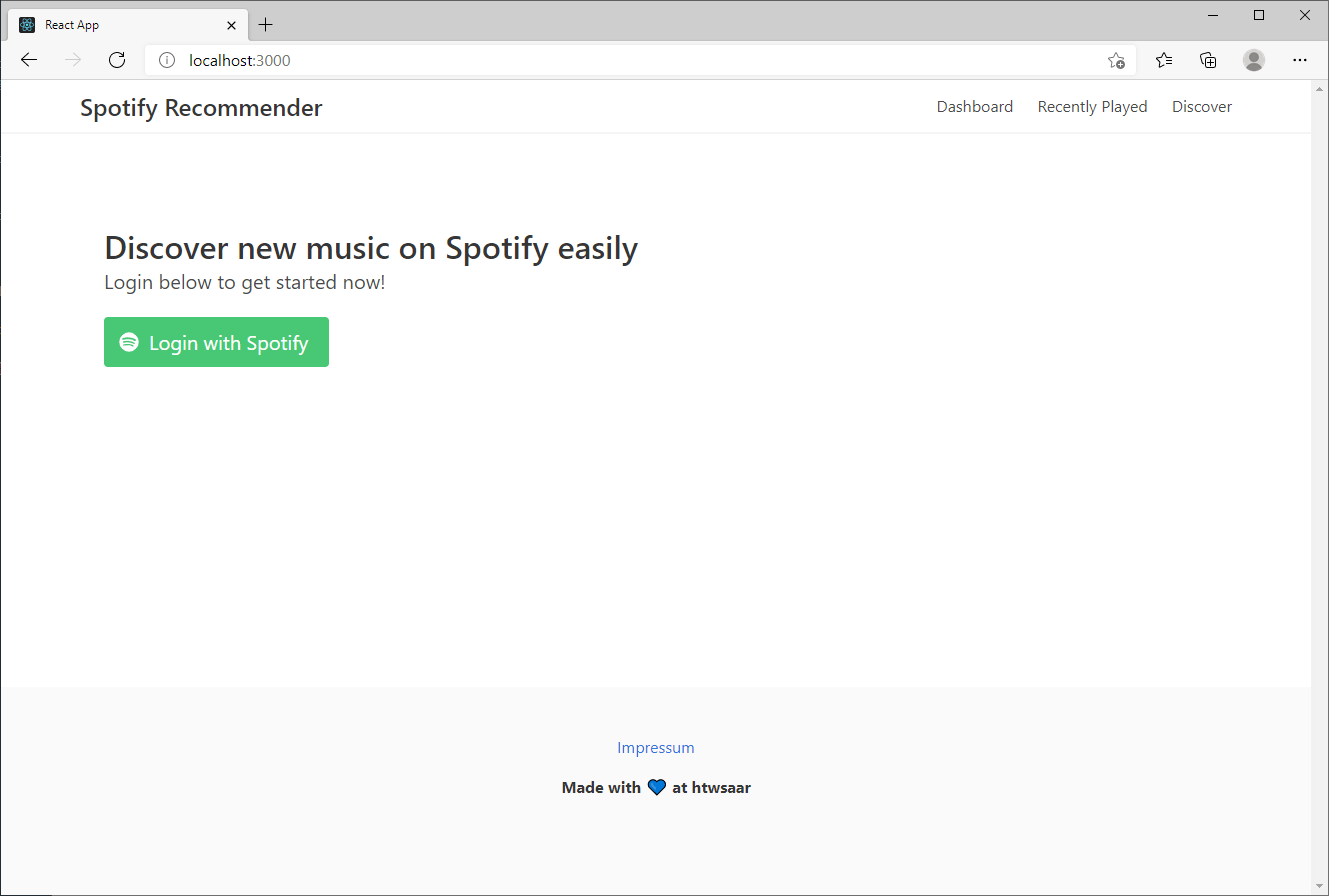
\includegraphics[width=1.0\textwidth]{Graphics/Chapter5/login-page.png}
    \caption{Login page after successful application start}
\end{figure}

\section{Known Issues}

\subsection{User remains logged-in in frontend even though he is not}

If your backend session expires, e.g. in case of restarting the backend or simply reaching the session expiration date, frontend will think that you are still logged-in even though you are not. This issue occurs if you do not logout using the \textit{Logout} button. As a consequence, the user object remains cached in local storage of the browser. You will still be able to open pages that require login but opening the browser console will reveal errors. To fix this issue, logout in the frontend and login again.

\subsection{Backend application will not start using Java 16}

Although newer Java versions, more often than not, are compatible with older ones, Java 16 breaks compatibility with a heavily used dependency called Project Lombok. This is because of JEP 396 (Strongly Encapsulate JDK Internals by Default) and will likely be fixed by a future Lombok update. As of now (Spring Boot 2.4.4) the backend application will not start using Java 16.
